\clearpage
\appendices
% Appendix tables/figures labeled A1, A2, B1... (section letter + local counter)
\makeatletter
\@addtoreset{table}{section}
\@addtoreset{figure}{section}
\makeatother
\renewcommand{\thetable}{\thesection\arabic{table}}
\renewcommand{\thefigure}{\thesection\arabic{figure}}

\section{Methodology Details}
\label{app:method_details}

\subsection{Glossary of Key Terms}
\label{app:glossary}

Table~\ref{tab:glossary} defines domain-specific terminology used throughout the paper.

\begin{table}[H]
\caption{Domain-specific terminology.}
\label{tab:glossary}
\centering
\small
\renewcommand{\arraystretch}{1.05}
\resizebox{\columnwidth}{!}{%
\begin{tabular}{p{2.0cm}p{5.4cm}}
\toprule
\textbf{Term} & \textbf{Definition} \\
\midrule
Token & Image patch embedded as $d$-dimensional vector; 197 tokens per $224{\times}224$ image \\
FFN & Feed-forward network: two-layer MLP applied per token in each transformer block \\
Expert & Routed residual branch processing a token subset; in CLEAR-MoE, all residual experts share one direction $(W_2{-}W_\text{shared})$ and differ only by a cluster-conditioned scalar $s_e$ \\
Router/Gate & Lightweight network mapping each token to a probability distribution over experts \\
MoE layer & FFN replaced by $E$ experts plus a router; only top-$k{<}E$ experts activate per token \\
SVD & Singular value decomposition; truncated SVD retains top-$r$ singular components \\
$k$-means & Partitions $N$ points into $k$ clusters by minimising within-cluster variance \\
Calibration set & Small representative set used to measure model statistics (no weight updates) \\
AI & Arithmetic intensity: FLOPs per byte of memory accessed \\
Ridge point & AI where compute ceiling equals memory bandwidth ceiling (21.4 FLOPs/B on GTX\,960) \\
p50 Latency & Median over 100 repeated forward passes; robust to OS-scheduling outliers \\
cuBLAS & NVIDIA's optimised linear-algebra library; batched GEMM calls dispatch through it \\
\bottomrule
\end{tabular}
}
\end{table}

\FloatBarrier
\subsection{Dataset Preparation and EDA}
\label{app:eda}

\textbf{Imagenette.} 13,394 raw images were scanned using SHA-256 deduplication, robust z-score filtering ($\tau{=}3.5$), and Isolation Forest (contamination\,=\,0.01). 118 images (0.88\%) were removed, yielding a clean set of 9,391 train / 3,885 val (used for EDA analysis only). The \emph{standard} Imagenette validation split (3,925 images, including the 40 removed as anomalies by our filter) was used for all reported Top-1 accuracy evaluation, ensuring comparability with prior work. ImageNet normalisation and Lanczos-4 resize to $224{\times}224$ are applied.

\textbf{Distribution shift analysis.} DeiT-Small penultimate activations for all 3,885 clean val images (shape $3885{\times}384$): PSI\,=\,0.043 ($<$0.1, negligible shift), JSD\,=\,0.018, KS $p$-values\,$>$0.05 for all 10 classes. \textbf{Clustering quality.} $k{=}10$ on penultimate image-level activations: Silhouette\,=\,0.542, Davies-Bouldin\,=\,1.24, confirming that the feature space supports class-level cluster separation. Note that CLEAR-MoE clusters token-level intermediate activations with $k{=}4$, which is a complementary but distinct analysis; the image-level EDA establishes feature quality rather than directly validating token cluster assignments. \textbf{SVD energy.} Rank-192 truncation retains 99.2\% of penultimate activation matrix variance; top-10 singular values capture 67.8\%. The effect of $W_2$ truncation rank on accuracy and reconstruction error is evaluated in Table~\ref{tab:rank_sweep}.

Table~\ref{tab:eda} summarises these preprocessing and analysis statistics.

\begin{table}[H]
\caption{Dataset preprocessing and EDA statistics.}
\label{tab:eda}
\centering
\small
\resizebox{\columnwidth}{!}{%
\begin{tabular}{p{3.5cm}p{4.0cm}}
\toprule
\textbf{Statistic} & \textbf{Value} \\
\midrule
Raw Imagenette images & 13,394 \\
Removed (anomalous) & 118 (0.88\%) \\
Train / val split & 9,391 / 3,885 (clean, EDA only); 3,925 (standard, used for all Top-1) \\
Train-test PSI & 0.043 ($<$0.1 = negligible shift) \\
Train-test JSD & 0.018 \\
$k{=}10$ Silhouette score & 0.542 \\
$k{=}10$ Davies-Bouldin & 1.24 \\
Rank-192 SVD variance & 99.2\% \\
Calibration size & 200 images \\
\bottomrule
\end{tabular}
}
\end{table}


\FloatBarrier
\subsection{Algorithm Pseudocode}
\label{app:algorithms}

Algorithms~\ref{alg:scoring}--\ref{alg:inference} give pseudocode for the three core CLEAR-MoE phases.

\begin{algorithm}[H]
\caption{Phase 2: Layer Scoring and Selection}
\label{alg:scoring}
\begin{algorithmic}[1]
\REQUIRE Calibration activations $\{h_l^{(i)}\}$, $L$\,=\,12 layers, select $k{=}6$
\FOR{each layer $l$}
  \STATE $\text{sp}(l) \gets \frac{\sum_j \mathbf{1}(|h_{l,j}|<0.01)}{\operatorname{numel}(h_l)}$
  \STATE $\text{cl}(l) \gets \text{Silhouette}(k\text{-means}(h_l, E))$
  \STATE $\text{se}(l) \gets \|\Delta\text{logits}\|/\|\text{logits}\|$ \hfill (zero FFN output)
  \STATE $\mathcal{S}(l) \gets 0.4\,\text{sp} + 0.4\,\text{cl} - 0.2\,\text{se}$
\ENDFOR
\STATE Select top-$k$ layers by $\mathcal{S}$
\end{algorithmic}
\end{algorithm}

\begin{algorithm}[H]
\caption{Phase 3: Expert Extraction (fc1 shared; fc2 decomposed)}
\label{alg:extraction}
\begin{algorithmic}[1]
\REQUIRE $W_2 \in \mathbb{R}^{d \times d_\text{ffn}}$, activations $z$, $E$, rank $r$
\STATE $[U,\Sigma,V] \gets \text{SVD}(W_2)$; \; $W_\text{shared} \gets U_r\Sigma_r V_r^\top$
\STATE $\{C_1,\ldots,C_E\} \gets k\text{-means}(z, E)$
\FOR{$e \in \{1,\ldots,E\}$}
  \STATE $s_e \gets \frac{\frac{1}{|C_e|}\sum_{i\in C_e}\|z_i\|_2}{\frac{1}{N}\sum_{i=1}^{N}\|z_i\|_2}$
  \STATE $W_e^\text{res} \gets (W_2 - W_\text{shared}) \cdot s_e$
\ENDFOR
\end{algorithmic}
\end{algorithm}

\begin{algorithm}[H]
\caption{CLEAR-MoE FFN Inference (Grouped backend)}
\label{alg:inference}
\begin{algorithmic}[1]
\REQUIRE Tokens $x$, shared fc1, $W_\text{shared}$, $\{W_e^\text{res}\}$, Router $g$
\STATE $z \gets \text{GELU}(\text{fc1}(x))$ \hfill (shared, all tokens)
\STATE $h_\text{sh} \gets z W_\text{shared}^\top$ \hfill (shared SVD basis)
\STATE $a \gets \text{argmax}(g(x))$ \hfill (expert assignment)
\STATE Sort $z$ by $a$; get sub-batch boundaries via index search
\STATE $h_\text{res}[e] \gets z_e W_e^{\text{res}\top}$ for each expert $e$
\STATE Unshuffle $h_\text{res}$; $y \gets h_\text{sh} + h_\text{res}$
\end{algorithmic}
\end{algorithm}


\FloatBarrier
\section{Experimental Configuration}
\label{app:experimental_config}

\subsection{Hardware and Software Setup}
\label{app:setup}

Table~\ref{tab:setup} lists the complete hardware and software configuration used in all experiments.

\begin{table}[H]
\caption{Hardware and software configuration for all experiments.}
\label{tab:setup}
\centering
\small
\resizebox{\columnwidth}{!}{%
\begin{tabular}{p{3.0cm}p{4.5cm}}
\toprule
\textbf{Item} & \textbf{Specification} \\
\midrule
OS & Windows 11 Pro \\
GPU & NVIDIA GeForce GTX\,960 \\
GPU memory & 4.0\,GB GDDR5 \\
Memory bandwidth & 112\,GB/s \\
Peak FP32 throughput & 2.4\,TFLOP/s \\
Ridge point & 21.4\,FLOPs/Byte \\
CUDA & 11.8 \\
PyTorch & 2.6.0+cu118 \\
Classification backbone & DeiT-Small; 22M parameters; patch size 16$\times$16; $d{=}384$; $d_\text{ffn}{=}1536$; 12 transformer blocks \\
Segmentation backbone & Not evaluated (planned future work) \\
Default $E$ & 4 experts \\
Default rank $r$ & $r{=}d/2{=}192$ for DeiT-Small (50\% of matrix rank) \\
Calibration size & 200 images \\
Router training & 5 epochs, AdamW, lr\,$10^{-3}$, cosine decay \\
Latency & p50 of 100 passes, batch\,=\,8, \texttt{cuda.synchronize()} \\
\bottomrule
\end{tabular}
}
\end{table}

\FloatBarrier
\section{Extended Experimental Results}
\label{app:extended_results}

\subsection{Full Ablation Tables}
\label{app:ablation}

\textbf{Per-layer composite scores.} Full composite scores for all 12 DeiT-Small FFN blocks appear in Table~\ref{tab:layer_scores_main} (Section~\ref{sec:method}). Block~0 ranks last (composite\,=\,0.101) due to sensitivity\,=\,0.946.

\textbf{Full layer-selection policy ablation.} The complete L0--L10 ablation now appears in Table~\ref{tab:ablation} (Section~\ref{sec:ablation}).

\FloatBarrier
\subsection{Hyperparameter Sensitivity Studies}
\label{app:sensitivity}

Tables~\ref{tab:seeds}--\ref{tab:router_comparison} report the full numerical results for the five hyperparameter sensitivity studies summarised in Section~\ref{sec:results}.

\begin{table}[H]
\caption{3-Seed Robustness. Full composite-score pipeline, $E{=}4$, DeiT-Small.}
\label{tab:seeds}
\centering
\small
\resizebox{\columnwidth}{!}{%
\begin{tabular}{lrrrr}
\toprule
\textbf{Seed} & \textbf{Top-1} & \textbf{p50 ms} & \textbf{Router Acc} & \textbf{Skew} \\
\midrule
42  & 86.68\% & 85.05 & 0.925 & 0.099 \\
123 & 86.70\% & 83.90 & 0.928 & 0.116 \\
456 & 86.73\% & 78.89 & 0.928 & 0.101 \\
\midrule
\textbf{Mean$\pm$Std} & \textbf{86.70$\pm$0.02\%} & 82.6$\pm$2.7 & 0.927$\pm$0.002 & 0.105$\pm$0.008 \\
\bottomrule
\end{tabular}
}
\end{table}

\begin{table}[H]
\caption{Calibration-set sensitivity. Multiple random subsets per size.}
\label{tab:calib}
\centering
\small
\resizebox{\columnwidth}{!}{%
\begin{tabular}{rrrrrr}
\toprule
$N_\text{cal}$ & \textbf{Sub.} & \textbf{Top-1} & \textbf{Router Acc} & \textbf{Skew} \\
\midrule
 50 & 1 & 86.70\% & 0.867 & 0.139 \\
 50 & 2 & 86.68\% & 0.833 & 0.073 \\
 50 & 3 & 86.65\% & 0.856 & 0.139 \\
100 & 1 & 86.55\% & 0.896 & 0.094 \\
100 & 2 & 86.60\% & 0.908 & 0.150 \\
100 & 3 & 86.70\% & 0.899 & 0.153 \\
200 & 1 & 86.68\% & 0.926 & 0.099 \\
200 & 2 & 86.60\% & 0.928 & 0.128 \\
500 & 1 & 86.70\% & 0.953 & 0.098 \\
\bottomrule
\end{tabular}
}
\end{table}

\begin{table}[H]
\caption{SVD rank sweep. Seed~42, $E{=}4$, composite scoring.}
\label{tab:rank_sweep}
\centering
\small
\begin{tabular}{rrrr}
\toprule
\textbf{Rank $r$} & \textbf{Top-1} & \textbf{p50 ms} & \textbf{Recon Err} \\
\midrule
 16 & 86.75\% & 78.13 & 0.907 \\
 32 & 86.65\% & 76.79 & 0.841 \\
 64 & 86.65\% & 76.60 & 0.734 \\
 96 & 86.75\% & 78.07 & 0.643 \\
128 & 86.68\% & 77.82 & 0.562 \\
192 & 86.62\% & 76.01 & 0.420 \\
256 & 86.70\% & 77.36 & 0.294 \\
\bottomrule
\end{tabular}
\end{table}

\begin{figure}[H]
\centering
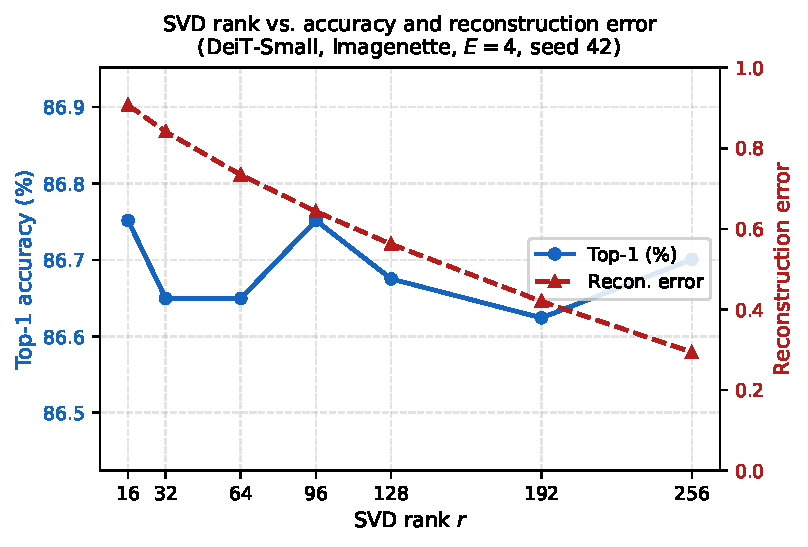
\includegraphics[width=0.85\columnwidth]{../figures/rank_sweep.pdf}
\caption{SVD rank vs.\ Top-1 accuracy (left axis, blue) and reconstruction error (right axis, red). Accuracy spans 0.13\,pp across $r\in\{16,\ldots,256\}$ while reconstruction error drops from 0.907 to 0.294, confirming rank does not gate accuracy once the shared basis captures the dominant singular subspace.}
\label{fig:rank_sweep}
\end{figure}

\begin{table}[H]
\caption{Expert-count study. Seed~42, composite scoring, $k{=}6$.}
\label{tab:expert_count}
\centering
\small
\begin{tabular}{rrrrrr}
\toprule
$E$ & \textbf{Top-1} & \textbf{p50 ms} & \textbf{Rtr Acc} & \textbf{Skew} & \textbf{Empty} \\
\midrule
 2 & 86.65\% & 73.4 & 0.967 & 0.247 & 0 \\
 4 & 86.65\% & 77.5 & 0.923 & 0.074 & 0 \\
 8 & 86.80\% & 84.3 & 0.893 & 0.042 & 0 \\
16 & 86.39\% & 97.8 & 0.865 & 0.024 & 0 \\
\bottomrule
\end{tabular}
\end{table}

\begin{table}[H]
\caption{Router architecture comparison. Seed~42, $E{=}4$, composite scoring. Entropy: aggregate expert-usage entropy (distribution of tokens across experts, per layer; max $=\ln 4 \approx 1.386$). Note: this is the \emph{load-balance} entropy, distinct from the per-token predictive entropy in Fig.~\ref{fig:expert_entropy} ($\approx$0.40 nats), which measures router confidence.}
\label{tab:router_comparison}
\centering
\small
\resizebox{\columnwidth}{!}{%
\begin{tabular}{lrrrrrrr}
\toprule
\textbf{Router} & \textbf{Top-1} & \textbf{p50 ms} & \textbf{Rtr Acc} & \textbf{Skew} & \textbf{Entropy} & \textbf{Params} \\
\midrule
Linear   & 86.68\% & 78.0 & 0.925 & 0.099 & 1.296 & 9,240 \\
MLP      & 86.68\% & 75.6 & 0.980 & 0.095 & 1.300 & 149,400 \\
Adaptive & 86.68\% & 77.6 & 0.936 & 0.099 & 1.296 & 9,240 \\
\bottomrule
\end{tabular}
}
\end{table}

\FloatBarrier
\subsection{Dispatch Benchmark and Parallel Scaling}
\label{app:dispatch}

Table~\ref{tab:dispatch} benchmarks all three CUDA backends under four token-load imbalance levels ($B{=}8$, $T{=}1568$ tokens, $E{=}4$, GTX\,960); CPU Serial is included as a baseline, allowing direct GPU-vs-CPU comparison at each imbalance level. The roofline plot appears in Fig.~\ref{fig:roofline} (Section~\ref{sec:results}). Table~\ref{tab:parallel} projects multi-device throughput analytically.

\begin{table}[H]
\caption{Dispatch micro-benchmark: p50 latency (ms) and throughput (K\,tok/s) across imbalance levels. $T{=}1568 = 8{\times}196$ tokens (class token excluded from expert dispatch; processed on the dense path). Calibration uses 197 tokens/image including the class token.}
\label{tab:dispatch}
\centering
\footnotesize
\setlength{\tabcolsep}{3pt}
\resizebox{\columnwidth}{!}{%
\begin{tabular}{lrrrrrrrr}
\toprule
& \multicolumn{2}{c}{\textbf{0\% imb.}} & \multicolumn{2}{c}{\textbf{40\% imb.}} & \multicolumn{2}{c}{\textbf{60\% imb.}} & \multicolumn{2}{c}{\textbf{80\% imb.}} \\
\cmidrule(lr){2-3}\cmidrule(lr){4-5}\cmidrule(lr){6-7}\cmidrule(lr){8-9}
\textbf{Backend} & ms & K/s & ms & K/s & ms & K/s & ms & K/s \\
\midrule
CPU Serial & 6.01 & 261 & 7.22 & 217 & 5.96 & 263 & 5.96 & 263 \\
Naive       & 3.67 & 428 & 3.55 & 442 & 3.50 & 448 & 3.59 & 437 \\
Grouped     & 2.36 & 665 & 2.10 & 747 & 2.30 & 681 & 2.14 & 733 \\
cuBLAS      & \textbf{2.15} & \textbf{728} & 2.29 & 684 & 2.45 & 639 & 2.81 & 558 \\
\bottomrule
\end{tabular}
}
\end{table}

\begin{figure}[H]
\centering
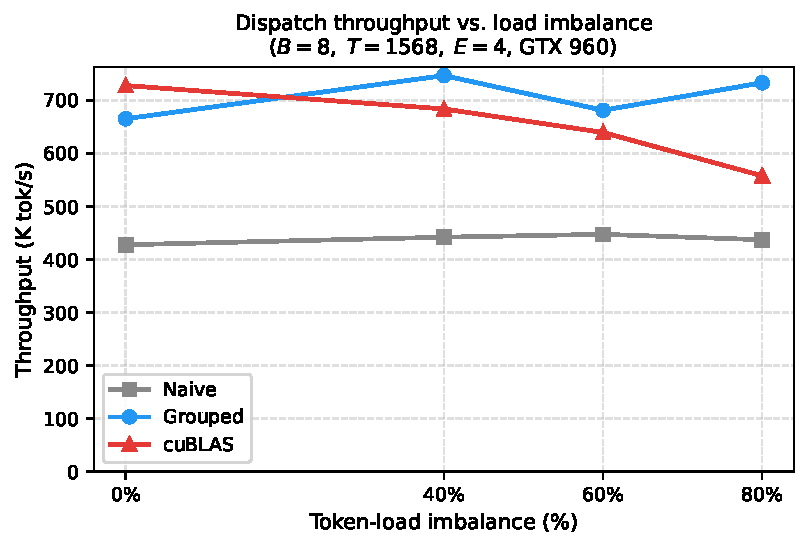
\includegraphics[width=0.85\columnwidth]{../figures/dispatch_curve.pdf}
\caption{Dispatch throughput vs.\ token-load imbalance for three CUDA backends ($B{=}8$, $T{=}1568$, $E{=}4$, GTX\,960). Grouped is stable across all imbalance levels (665--747\,K\,tok/s); cuBLAS degrades 23\% from 0\% to 80\% imbalance due to padding waste. For variable-load workloads, Grouped is the recommended backend.}
\label{fig:dispatch_curve}
\end{figure}

\textbf{GPU vs.\ CPU and Parallel Scaling.}
\label{app:parallel}

GPU vs.\ CPU speedup at balanced load is readable from the CPU Serial row in Table~\ref{tab:dispatch} above: at 0\% imbalance, cuBLAS achieves 728\,K\,tok/s vs.\ 261\,K\,tok/s for CPU Serial ($2.79\times$ speedup).

\textbf{Multi-device projection (simulated; no second GPU available).} All-to-all and AllReduce costs are modelled analytically using PCIe Gen3$\times$16 bandwidth (16\,GB/s). Results are \emph{not} measured NCCL runs.

\begin{table}[H]
\caption{Parallel scaling projection. Expert/Data/Pipeline parallelism are simulated; single-GPU is measured.}
\label{tab:parallel}
\centering
\small
\resizebox{\columnwidth}{!}{%
\begin{tabular}{lrrrr}
\toprule
\textbf{Mode} & \textbf{tok/s} & \textbf{Devices} & \textbf{Speedup vs GPU-1} & \textbf{Efficiency} \\
\midrule
Full-model single-GPU  & 225K & 1 & 1.00$\times$ & 1.00 \\
Expert Parallel EP-2 (sim.) & 175K & 2 & 0.78$\times$ & 0.39 \\
Pipeline Parallel PP-2 (sim.) & 8K & 2 & 0.03$\times$ & 0.02 \\
\bottomrule
\multicolumn{5}{l}{\footnotesize All multi-device entries are simulated via PCIe Gen3$\times$16 bandwidth; no NCCL runs performed.} \\
\multicolumn{5}{l}{\footnotesize EP-2 overhead: all-to-all token redistribution (AI\,=\,0.1\,F/B).} \\
\multicolumn{5}{l}{\footnotesize PP-2: 50\% pipeline bubble with 1 micro-batch, 2 stages.} \\
\multicolumn{5}{l}{\footnotesize Single-GPU throughput is full-model (distinct from dispatch-only throughput in Table~C6).} \\
\end{tabular}
}
\end{table}

